%!TEX root = thesis.tex

%%%%%%%%%%%%%%%%%%%%%%%%%%%%%%%%
% intro.tex: Introduction to the thesis
%%%%%%%%%%%%%%%%%%%%%%%%%%%%%%%%
\chapter{Introduction}
\label{chap:intro}


A galaxy's morphology is the culmination of its formation, interactions, and evolution through environmental as well as internal processes. It is a snapshot into the current state of a galaxy's life as well as window to its past. Though sometimes subtle, the insights gleaned through the study of galaxy morphology have radically changed our view of universe since the time of Edwin Hubble. 


Astronomers have made use of visual galaxy morphologies to understand the dynamical structure of these systems for nearly ninety years 
\citep[e.g.,][]{Hubble1936, 
			deVauc1959, 
			Sandage1961, 
			vandenBergh1976, 
			NairAbraham2010, 
			Baillard2011}. 
The division between early-type and late-type systems corresponds, for example, to a wide range of parameters from mass and luminosity, to environment, colour, and star formation history 
\citep[e.g.,][]{Kormendy1977,  
			Dressler1980, 
			Strateva2001, 
			Blanton2003, 
			Kauffman2003, 
			Nakamura2003, 
			Shen2003, 
			Peng2010}; 
while detailed observations of morphological features such as bars and bulges provide information about the history of their host systems 
\citep[e.g., review by][]{KK04, 
			Elmegreen2008, 
			Sheth2008, 
			Masters2010, 
			Simmons2014}. 
Modern studies of morphology  divide systems into broad classes 
\citep[e.g.,][]{Conselice2006, 
			Lintott2008, 
			Kartaltepe2015, 
			Peth2016}, 
but a wealth of information can be gained from identifying new and often rare classes, such as low redshift clumpy galaxies \citep[e.g.,][]{Elmegreen2013}, polar-ring galaxies \citep[e.g.,][]{Whitmore1990}, and the green peas \citep{Cardamone2009}. 

Obtaining these morphologies has traditionally been a time-consuming visual endeavor and only in the past twenty years have automated morphological assignment been possible. Even with the varied automated approaches currently being exploited, an era of Even Bigger Data looms for the field of astronomy. The next decade will herald the first light of more powerful ground- and spaced-based telescopes such as the Large Synaptic Survey Telescope (LSST), Euclid, and WFIRST. The surveys planned for these instruments promise to revolutionize the field of astrophysics providing several orders of magnitude more data than all of Everything? I don't know. Traditional techniques will not be sufficient for extracting galaxy morpholgoies on a pertinent timescale. 

This thesis details a solution to the scalability of galaxy morphology designations by examinging classification obtained as part of the Galaxy Zoo project, a crowd-sourcing initiative that has obtained morphological classifications from over a million volunteers for over a million galaxies from several surveys. Though innovative, even crowd-sourcing will be unable to sustain the classification load for future surveys. Instead, these classifications are combined with supervised machine learning algorithms that train on automated measurements of galactic morphological structural indicators. This thesis begins with a detailed account of the methodology used to obtain these morphological structural indicators (Chapter \ref{chap:2}). Chapter \ref{chap:3} demonstrates how crowd-sourcing techniques can be optimized by applying SWAP [come up with generic words] to Galaxy Zoo classifications, while Chapter \ref{chap:4} explores the combination of visual classifications with machine learning algorithms. Also included is a prelimary analysis of a rare sample of ``clumpy'' galaxies in the local universe discovered during the course of the analysis of Galaxy Zoo classifications [NOT GOOD WORDS] (Chapter \ref{chap:5}). While common in the distant universe, these potential local counterparts could shed light on  star-formation things and stuff. This Introduction provides a brief overview of galaxy formation, the sciece of morphology, and galaxy classification techniques, as well as an overview of Galaxy Zoo: Express, an integrated framework of human and machine galaxy classifiers. 




\section{Galaxy formation}
Brief overview of how galaxies form and the dizzying variety of morphologies. 


\section{Standard morphology designations}
\begin{figure}
\centering
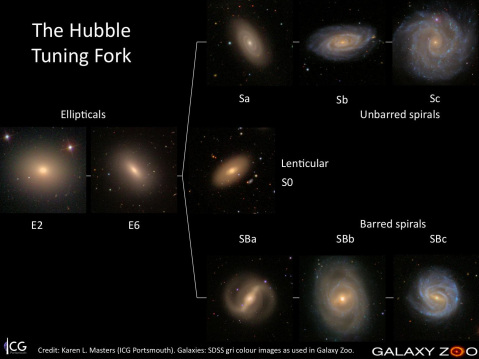
\includegraphics[width=4.5in]{Figures/Masters_tuningfork.jpg}
\caption[Hubble tuning fork]{i'm a caption}
\label{fig: tuning fork}
\end{figure}

The oldest and arguably simplest system for categorizing galaxy morphology dates back to the 1930s and Edwin Hubble's famous ``tuning fork''. Based on a small sample, Hubble classified galaxies into two major groups, elliptical and spiral. Visually, elliptical galaxies possessed a smooth light distribution while spirals are characterized by well-defined disk structure with spiral arms. Hubble assigned a number to elliptical galaxies denoting the degree of their ellipticity, where 0 corresponds to a nearly perfectly round galaxy and 7 being highly elongated. Spirals were given additional designation in the form of letters a through c, characterizing the compactness of their spiral arms. For example, ``Sa'' galaxies are tightly wound, whereas "Sc" spirals are looser. The spiral category was then further subdivided by galaxies that exhibited a central bar. There is also indications that the bulges inherent to many spiral galaxies share a close connection to elliptical galaxies. 

It became common to call galaxies on the left side of the diagram ``early-types,'' and those on the right ``late-types''. Contrary to this author's belief, Hubble never intended these designations to imply galactic evolution. Instead, this terminology was borrowed from stars, where massive O and B stars were referred to as ``early-type'', while older stars were known as ``late-type''\citep{Buta2011}. It has subsequently become clear that, much to the contrary, ellipticals are dominated by late-type stars while disk galaxies are typically composed of young, early-type stars.  Unfortunately, the misnomer has stuck. 

%This hybrid category, denoted S0 on the tuning-fork diagram, was originally thought to be a transition stage between these two fundamental galaxy types. Additionally, it was surmised that galaxies travelled along the Hubble tuning fork from left to right. While this theory has literally been turned on its head, astronomers are unfortunately left with the misnomer of ``early-'' and ``late''-type galaxies referring to ellipticals and spirals respectiively. 


This method of galaxy classification was based on an extremely small sample of which only a few percent did not conform to the basic designations originally posited by Hubble. These leftover galaxies were dubbed ``Irregulars'' or ``peculiars''. It wasn't until much later that it was discovered these types of galaxies are far more prevalant than Hubble originally thought. Since this early attempt at classification, several other systems have been put forward but most share the same basic categories. Indeed, even this simplistic approach has yielded nearly a hundred years of science that has advanced our understanding of galaxy formation, structure, and evolution. 
 


\section{Morphology as a tracer of galaxy evolution}
Though simple, these basic categories have proved to then segue into how those different morphologies provide detailed insights into formation and evolution. Give examples of the science that can be gleaned from broad classifications (early- vs late-type galaxies), and how rare classifications can provide unique viewpoints (clumpy galaxies at low redshift, or green peas, i.e.)

Any theory of galaxy formation and evolution will
have to, at some point, account for the bewildering array of galactic forms. --Buta
 Galaxy morphology is strongly correlated with galactic star formation history. Galaxies
where star formation ceased gigayears ago tend to look very different from those where star
formation continues at the present time. 


\subsection{Stellar populations and star-formation histories}
At its heart, morphology simply traces an integrated 2D projection of a galaxy's light distribution. As such, it encodes information on the distribution of a galaxy's stellar, gas, and dust content. However, these components are best traced through different wavelengths of light. 

Consider a coevolving stellar population with a mass distribution according to your favorite initial mass function. Stars on the Main Sequence (MS) radiate in the blue and ultraviolet (UV) end of the spectrum due to their high effective temperatures. The most massive quickly evolve off the MS and become red supergiants causing a decrease in the UV flux and an increase in the near infrared (NIR). As the low mass stars in this stellar population continue to evolve off the MS, the UV flux steadily decreases until eventually the red giant branch becomes the dominant source of flux, radiating in the IR. This so-called \textit{passive} evolution indicates that as a galaxy ages it becomes redder. A galaxy's morphology is tightly correlated with its color: massive elliptical galaxies are typically referred to as ``red and dead,'' possessing old stellar populations, while disk galaxies are generally still undergoing star formation and thus possess young, bluer stellar populations \citep[e.g.,][]{Strateva2001,Baldry2004b, Cirasuolo2007, Lee2013, Taylor2015}. This dichotomy is so prBevalent that color has been used as a proxy for morphology when acquiring the latter was impractical \citep[e.g.,][]{Shen2003, Blanton2003c}. 

Furthermore, this color bimodality correlates with luminosity resulting in the color-magnitude relation (CMR) \citep{Baldry2004a, Bell2004}. Now ubiquitous, this relation visualizes the separation of galaxy colors as a function of luminosity resulting in three main categories: the blue cloud, the red sequence and, more recently recognized, the green valley. Studies have shown that the red sequence is dominated by early-type galaxies like elliptical/S0 while disk galaxies reside in the blue cloud. There is a distinct gap between these two galaxy populations but recent studies have shown that, though sparse, galaxies also reside here. The top panel of Figure XXX \citep[credit:][]{Kormendy2012} shows an example of the color-magnitude relation for a sample of SDSS galaxies while the bottom panel depicts a schematic of the associated morphologies. 

\begin{figure}
\centering
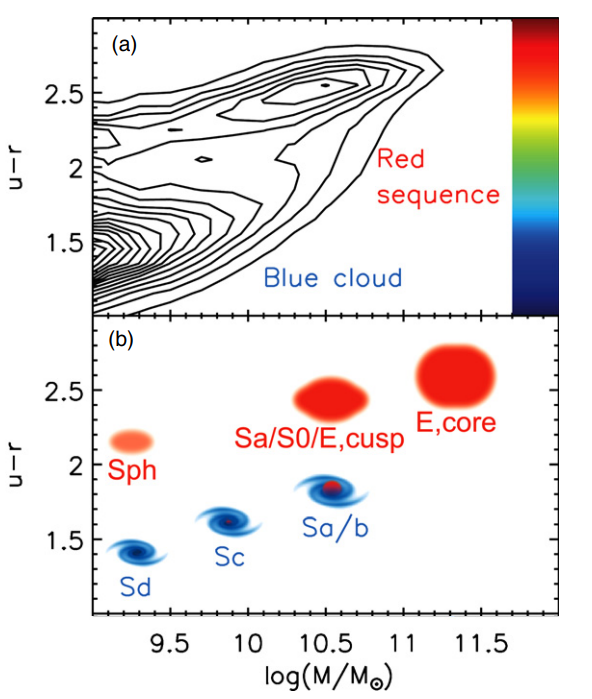
\includegraphics[width=3.5in]{Figures/kormendy_CMR.png}
\caption{Color-magnitude (mass) relation schematic \citep[credit:][]{Kormendy2012}.}
\end{figure}

For early-type galaxies, the color-magnitude relationship is more significant and provides a tool to constrain the star-formation histories of this galaxy population \citep{Sandage1978, Tully1982}. There exists a degeneracy between the age and metallicity of stellar populations: though older stars tend to be redder, this effect can also be achieved through an increase in stellar metallicity. It is now believed that the slope of the CMR is due primarily to metallitcy effects \citep{Bower1992, Kodama1997}, which then allows for age estimates to be placed on the last episode of significant star formation in early-type galaxies \citep[e.g.,][]{LopezCruz2004}. The small scatter in this relation reflects that these galaxies have old, passively evolving stellar populations. 

put this somewhere \citep{Mei2009}
%Galaxies contain more than just stars; gas and dust can also alter a galaxy's morphology. Dust is thought to be produced in AGB stars and distributed to the interstellar medium via stellar winds. Disk galaxies typically have more dust than ellipticals indicating that early-type galaxies expelled their dust content via dramatic mergers \citep{some people}. Blue light is more strongly attenuated than red light. This causes the dust to heat and radiate in the IR making a galaxy appear redder than it would otherwise. Another, more dramatic example of dust's effect on a galaxy's morphology is the dust lanes exhibited by many spiral galaxies. 

%It is clear that to fully understand a galaxy's composition, studying the morphology through observations across the electromagnitic spectrum is necessary: cold dust indicative of recent galaxy-galaxy interaction can be determine through radio observations of HI gas; infrared observations shed light on the dust content and old stellar components, visual and UV observations trace ever stellar nurseries, and high energy observations like X-rays give a tantalizing peak at what lurks in the bulges of active galaxies. 


\subsection{Mass and luminosity functions and galactic growth}
The most fundamental characteristic of a galaxy is its mass, however, this is a difficult quantity to measure. Much easier, instead, is a measurement of a galaxy's luminosity which takes only an image to estimate. Because the luminosity is, in large part, an integration of stellar light, mass generally scales with luminosity. The correlation of morphology with luminosity thus also implies a dependence on galaxy mass. A cottage industry for decades, constructing mass and luminosity functions has provided insights into the build-up of baryonic mass over cosmic time. 
In priniciple, the star formation density at a given epoch should represent the integral of the SF density up to that redshift. 

Stellar mass functions (SMFs) are a key first-order observatble that allows one to statistically trace back the formation of stars in the universe. Comparison with predicted SMFs further constrains the mechanisms with which galaxies converst 

Nearly half of the stellar mass in the local universe resides in early-type galaxies with half in late-type disk structures \citep{Kelvin2014}. However, this was not always the case.  Prior to z of 2, Hubble type morphologies become vague and are dominated by pecular galaxies \citep{Dickenson2000,Papovich2005,Cameron2011,Conselice2005,Conselice2011,Buitrago2013}and thus considerable evolution has taken place since that epoch. It has been shown that the Hubble morphologies emerge between 1 < z < 3 indicating that the peculiar high-redshift systems settle down into the galaxies we see in the local universe \citep{Mortlock2013}. 

It has been postulated that these early galaxies' evolution is dominated by violent mergers into spheroidal systems\citep{Driver2013,Bluck2009,Man2012}. After redshift 2 the dominant mechanism for galaxy evolution switches to cold gas accretion and hence the formation of of disk galaxies \citep{Conselice2013}. Of course, these processes are also presumed to be mass-dependent with the most massive galaxies settling into the familar Hubble sequence more quickly than low-mass galaxies \citep{Buitrago2013,Conselice2011,Mortlock2013}

Understanding the rate of growth and distribution of baryonic mass in galaxies provides constraints on the mechanisms necessary to produce such observations. It is well known that there was a period of increased star formation at z>2 when many galaxies rapidly formed stars at rates not typically observed in the local universe. However this formation was not distributed equally among all galaxies and types and the subsequent evolution of the star formation density of the universe paints a picture in which.. blah blah blah. 

A z$\sim$2, most of the stellar mass density is in irregular galaxies \citep{HuertasCompany2016} but this drops with redshift until, in the local universe, irregulars only dominate the SF density in low-mass galaxies. The abundance of passive (early-type) galaxies steadily increases from z 4 up until the present epoch. 

The quenching of star formation produces the color bimodality of galaxies, is likely the cause of the decrease in the star-formation rate density in the universe since z of 2 and could also be associated with morphological transformations within galaxies. 

The shape of the SMFs of galaxies has a knee corresponding to a characteristic stellar mass around 10^10.7 which appears to be independent of redshift. This implies that galaies tend to cease forming stars at this characteristic mass. This takes place primarily at z > 1 because, at later times, there are more passive, early-type galaxies than late-type star-forming galaxies with this particular mass. 


Mass build up over cosmic time: galaxies grow differently based on their morphology. Bivariate mass-luminosity function. Shen2003. Ellipticals gain X amount of mass since z~1 but only gain how much in size? On the other hand, disks are entirely different... suggests different growth mechanisms demarcated by optical morphology. 

stellar mass functions for disks and spheriods \citep{Thanjavur2016,Bell2003}
mass assembly history \citep{Bundy2005, Taylor2015, Brinchmann2000}
luminosity and mass functions \citep{Blanton2003b, Blanton2001}


In heirarchical models, morphologies transform according to the mass characteristics of mergers. We find no evidence for any change in the mass density of
spiral galaxies, suggesting the merging of spiral galaxies into
elliptical galaxies between and the present cannot be a z = 1
dominant process. Moreover, the total stellar mass density
hardly increases over the range sampled. Both results support
the contention that most massive galaxies formed their stars
prior to or around . Lower mass galaxies remain active z = 1
to much more recent epochs, consistent with the “downsizing”
picture introduced by Cowie and collaborators. --Brinchmann and Ellis


\subsection{Morphology as a function of environment}
A galaxy's environment also has a direct relationship with its morphology. First quantified by \cite{Dressler1980}, the morphology-density relation is an emperical observation that elliptical galaxies tend to reside in the densest environments, i.e., rich groups and clusters, at all stages of cosmic time. in the richest and densest clusters of galaxies, the dominant morphology is elliptical, while for field galaxies, the dominant morphology is spiral. Furthermore, it's been determined that this relation evolves over time, at least for the densest environments. All of this points to scenarios in which the environment of a galaxy dictates, or influences its morphology and that the processes contributing to this effect have evolved with time. \citep[e.g.,][]{Fasano2000, Shen2003, Smith2005, Peng2010}

Much study has been done to separate the effects of environment from mass, i.e., secular, causes of morphological features. Peng, Shen,,etc. Cluster environments are, compared to the field, extremely hot and dense. Galaxies residing in these environments have faster velocity, on average. (What kind of v is that called again? I forgot.)  It's estimated that field galaxies are, on average, 1 per Mpc (?). The merging rate depends on the density of galaxies. In the past galaxies were closer together so merging was a bigger deal. Logically then, it would seem that merging happens all the timein clusters and that this then causes a morphological change from disk to elliptical. However, galaxies are moving so briskly in clusters that it becomes less likely that they collide! Instead, merging seems to be a predominant morphological mechanism in groups rather than clusters. In clusters, instead, other physical processes shape the way a galaxy evolves and looks over time. 

Spirals convert to S0/elliptical galaxies in clusters due to several processes: they should have lost their cold atomic and molecular gas via ram pressure stripping (but see Tonnesen \& Bryan 2009, for the effect of ram
pressure on molecular clouds), harassment (Moore et al. 1996),
strangulation (Kawata \& Mulchaey 2008), etc.


role of mergers CANDELS \citep{Karteltepe2010}
mergers and AGN \citep{Kocevski2012, Villforth2014}

\subsection{Insights from rare morophologies}
So far I've examined insights gleaned by considering large populations of galaxies split into broad categories of early- and late-types. Though unbeknownst to Hubble, it is now well known that galaxy structure and hence the integrated light profile is much more complicated and varied. Examing both finer galactic structure such as bars, as well as rare morphologies like the ``green peas'' has pushed the boundaries on our collective knowledge of galaxy evolution. What have we learned from the green peas? Clumpy galaxies at low redshift? Ring galaxies? 

-- insights concerning dynamical disks; star formation; blah. 


\section{Obtaining morphological designations}
Now that we all believe we should get these morphologies -- how should we do it? 

\subsection{Visual classifications}
The history of galaxy morphology assignment is rife with historical precendents due in large part to Edwin Hubble's original ``tuning fork.'' Seeing as Hubble originally thought these `nebulae' were features residing in our own galaxy, we end up with goofy shit where we call elliptcals ``early-type'' and disks ``late-type'' though subsequent studies all confirm that the ages of ellipticals are far older than those of spiral galaxies. 

Visual classification, though highly accurate due to the human mind's unique pattern recognition capability, is, however, entirely slow. Assignment of morphological type to galaxies thus resulted in small samples lacking statistical signifigance for decades (until the use of cartels of graduate students wherein morphologies for galaxy samples reached a few thousands). With surveys such as the Sloan Digital Sky Survey looming on the horizon, a new approach would be necessary in order to take advantage of the unique insights provided by galaxy morphologies.

This necessitated the birth of the Galaxy Zoo project, the first effort to crowd-source the task of galaxy morphology assignment to the general public. Blah blah blah Galaxy Zoo blah. 

While the Galaxy Zoo project has provided a solution that scales visual classification for current surveys  by harnessing the combined power of thousands of volunteers \citep{Lintott2008, Lintott2011, Willett2013, Willett2017, Simmons2017},  producing a prolific amount of scientific output \citep[e.g.,][]{Land2008, Bamford2009, Darg2010, Schawinski2014, Galloway2015, Smethurst2016}; upcoming surveys such as \textit{LSST} and \textit{Euclid} will require a different approach, imaging more than a billion new galaxies  \citep{LSST, Euclid}.  If detailed morphologies can be extracted for just  0.1\% of this imaging, we will have millions of images to contend with. A project of this magnitude would take more than sixty years to classify at Galaxy Zoo's current rate and configuration. Standard visual morphology 
methods will thus be unable to cope with the scale of data. 


Visual classification by experts: CANDELS \citep{Kartaltepe2015}

\subsection{Automated classifications}
Another approach has been the automated extraction of galaxy morpholgies with the development of both parametric and non-parametric structural indicators. 

It is well known that a galaxy's light profile can be modelled according to the function [insert function here] where the Sersic index, $n$, has been shown to correlate strongly with a distinction between early- and late-type galaxies. In particular, a Sersic index of $n=4$ corresponds to a de Vaucouleurs' profile which well describes the surface brightness of an elliptical galaxy as a function of its apparent radius from the galaxy's center. On the other hand, a Sersic index of $n=1$ describes an exponential profile which is a good description for spiral galaxies. 

A drawback to the parametric approach is the need to assume the underlying distribution and while this works technique works well for galaxies that are obviously elliptical or spiral, it produces mixed results for other morphological types, i.e., irregulars or peculiars, which have low central concentration resulting in a low Sersic index, but which do not have disks or spiral arms. 

Non-paramteric structural indicators require fewer assumptions on the data and are instead derived observationally. Several of these diagnostics have been developed over the past couple decades, each probing a different part of the galaxy's light profile and thus its overall dynamical distribution. The most common diagnostics are described below. 

Closely related to the Sersic index is the non-paramatric diagnostic of concentration. A galaxy's concentration aims to identify how dense a galaxy's central surface brightness profile is. Concentration, originally conceived by Abraham(?) has had several definitions over the years. The most common consider the ratio of the aggregated light within two concentric apertures about the galaxy's center. Typically, these apertures contain 50 and 90\% of the galaxy's light (another common approach is to use 50\% and 80\%). Because 


Example of using parametric Sersic profile to classify galaxies as early-/late-type:
``We show that the wavelength-dependence of n may be employed to separate visually-classified early- and late-type galaxies in a manner similar to the use of colour and n. Furthermore, we find that the wavelength variation of n can recover galaxies that are misclassified by these other morphological proxies."\citep{Vika2015}

Peng(?) [was that the first?] developed the first model to decompose a galaxy's light profile into 

The radial luminosity profile of a disk is usually exponential, with departures from an
exponential being due to the presence of other structures. --Buta

Another approach has been the automated extraction of morphologies with the development of parametric \citep{Sersic1968, Odewahn2002, Peng2002}, and non-parametric 
\citep{Abraham1994, 
	   Conselice2003, 
	   Abraham2003, 
	   Lotz2004,  
	   Freeman2013} 
structural indicators. While these scale well to large samples 
\citep[e.g.,][]{Simard2011, 
			Griffith2012, 
			Casteels2014, 
			Holwerda2014, 
			Meert2016}, 
they often fail to capture detailed structure and can provide only statistical morphologies with large uncertainties \cite[e.g.,][]{Abraham1996, Bershady2000}. 


\subsection{Machine learning}
Machine learning techniques are becoming increasingly popular for classification and image processing tasks. Another automated approach, these generally work by defining a set of features that describe the morphology in an $N$-dimensional space. The location in this morphology space defines a morphological type for each galaxy. Learning the morphology space can be achieved through algorithms such as Support Vector Machines \citep{HuertasCompany2008} or Principal Component Analysis \citep{Watanabe1985, Scarlata2007}. Another approach is through deep learning, a machine learning technique that attempts to model high level abstractions. Algorithms like convolutional and artificial neural networks (CNNs, ANNs) have been used for galaxy morphology classification with impressive accuracy 
\citep{Ball2004, 
	Banerji2010, 
	Dieleman2015, 
	HuertasCompany2015}. 
A drawback to all machine learning classification techniques is the need for standardized training data, with more complex algorithms requiring more data. Furthermore, these data must be consistent for each survey: differences in resolution and depth can be implicitly learned by the algorithm making their application to disparate surveys challenging. 


\section{Overview of Galaxy Zoo: Express}

 In this work we present a system that preserves the best features of both visual and automatic classifications, developing for the first time a framework that brings both human and machine intelligence to the task of galaxy morphology to handle the scale and scope of next generation data. We demonstrate the effectiveness of such a system through a re-analysis of visual galaxy morphology classifications collected during the Galaxy Zoo 2 project, and combine these with a Random Forest machine learning algorithm that trains on a suite of non-parametric morphology indicators widely used for automated morphologies. In this paper we focus on the first question of the Galaxy Zoo decision tree. We demonstrate that our method provides a factor of 11.4 increase in the rate of galaxy morphology classification  while maintaining at least 93.5\% classification accuracy as compared to Galaxy Zoo 2 published data. We first present an overview of our framework, which also serves as a blueprint for this paper. 


%%%-------------------------------------------------------
%%% FIGURE:     GZ EXPRESS Schematic
%%%-------------------------------------------------------
\begin{figure*}[ht!]
%\figurenum{1}
\plotone{Figures/human_machine/f1.pdf}
\caption[Schematic of the Galaxy Zoo: Express human+machine hybrid system.]{Schematic of our hybrid system. Humans provide classifications of galaxy images via a web interface. We simulate this with the Galaxy Zoo 2 classification data described in Chapter~\ref{chap:2}. Human classifications are processed with an algorithm described in Chapter~\ref{chap:3}. Subjects that pass a set of thresholds are considered human-retired (fully classified) and provide the training sample for the machine classifier as described in Chapter \ref{chap:4}. The trained machine is applied to all subjects not yet retired. Those that pass an analogous set of machine-specific thresholds are considered machine-retired. The rest remain in the system to be classified by either human or machine. This procedure is repeated  nightly. \label{fig: schematic}}
\end{figure*}


%%----------------------------------------------------------------------------------------------------------------------------------------------------
%%   GALAXY ZOO EXPRESS OVERVIEW
%%---------------------------------------------------------------------------------------------------------------------------------------------------

The Galaxy Zoo Express (GZX) framework combines human and machine to increase morphological classification efficiency, both in terms of the classification rate and required human effort. Figure~\ref{fig: schematic} presents a schematic of GZX including section numbers as a shortcut for the reader. We note that transparent portions  of the schematic represent areas of future work which we explore in Chapter \ref{chap:summary}. Any system combining human and machine classifications will have a set of generic features: a group of human classifiers, at least one machine classifier, and a decision engine which determines how these classifications should be combined.

In this work we demonstrate our system through a re-analysis of  Galaxy Zoo 2 (GZ2) classifications. This allows us to  create simulations of human classifiers. These classifications are used most effectively when processed with SWAP, a Bayesian code described in Chapter \ref{chap:3}, first developed for the Space Warps gravitational lens discovery project~\citep{Marshall2016}. These subjects provide the machine's training sample. 

In Chapter~\ref{chap:4}, we incorporate a machine classifier. We have developed a Random Forest algorithm that trains on measured morphology indicators such as Concentration, Asymmetry, Gini coefficient and \M{20} well-suited for the top-level question of the GZ2 decision tree, discussed in Chapter \ref{chap:2}. After a sufficient number of subjects have been classified by humans, the machine is trained and its performance assessed through cross-validation. This procedure is repeated nightly and the machine's performance increases with size of the training sample, albeit with a performance limit. Once the machine reaches an acceptable level of performance it is applied to the remaining galaxy sample. 

Even with this simple description, one can see that the classification process will progress in three phases.  First, the machine will not yet have reached an acceptable level of performance; only humans contribute to subject classification. Second, the machine's performance will improve; both humans and machine will be responsible for classification. Finally, machine performance will slow; remaining images will likely need to be classified by humans. This blueprint allows even modest machine learning routines to make significant contributions alongside human classifiers and removes the need for ever-increasing performance in machine classification.